% Fig. 1 — pipeline overview, drawn in TikZ and compiled to figures/fig1_pipeline.pdf.
%   pdflatex fig1_pipeline.tex      (or: latexmk -pdf fig1_pipeline.tex)
% Kept as a standalone document so the figure can be compiled, shared and iterated on
% without touching the paper. English text: the paper loads no CJK package.
%
% Red line (same as paper/fig1_pipeline.md): the figure only expresses the flow. Sample
% counts live in the text and tables, so they are deliberately absent here; if a count
% changes, this file does not go stale.
%
% Visual grammar: solid = main flow; dashed = check / optional / reuse path. The two
% quality gates (human review, independent-source dev benchmark) share one highlighted
% style because they are the two claims the paper leans on.
\documentclass[tikz,border=3pt]{standalone}
\usepackage[T1]{fontenc}
\usepackage{helvet}
\renewcommand{\familydefault}{\sfdefault}
\usepackage{tikz}
\usetikzlibrary{arrows.meta, positioning, fit, backgrounds, calc}

% Node text is short and centred, so hyphenation only makes it ragged.
\hyphenpenalty=10000
\exhyphenpenalty=10000

\tikzset{
  box/.style={draw, rounded corners=2pt, align=center, inner sep=4.5pt,
              line width=0.5pt, fill=blue!4, font=\small},
  arm/.style={box, fill=green!6, font=\footnotesize, anchor=north},
  gate/.style={draw, rounded corners=2pt, align=center, inner sep=4.5pt,
               line width=1.5pt, fill=orange!16},
  flow/.style={-{Latex[length=2.2mm, width=1.5mm]}, line width=0.7pt},
  plain/.style={line width=0.7pt},
  aux/.style={flow, dashed},
  tag/.style={font=\itshape\scriptsize, text=black!60, fill=white, inner sep=1pt},
}

\begin{document}
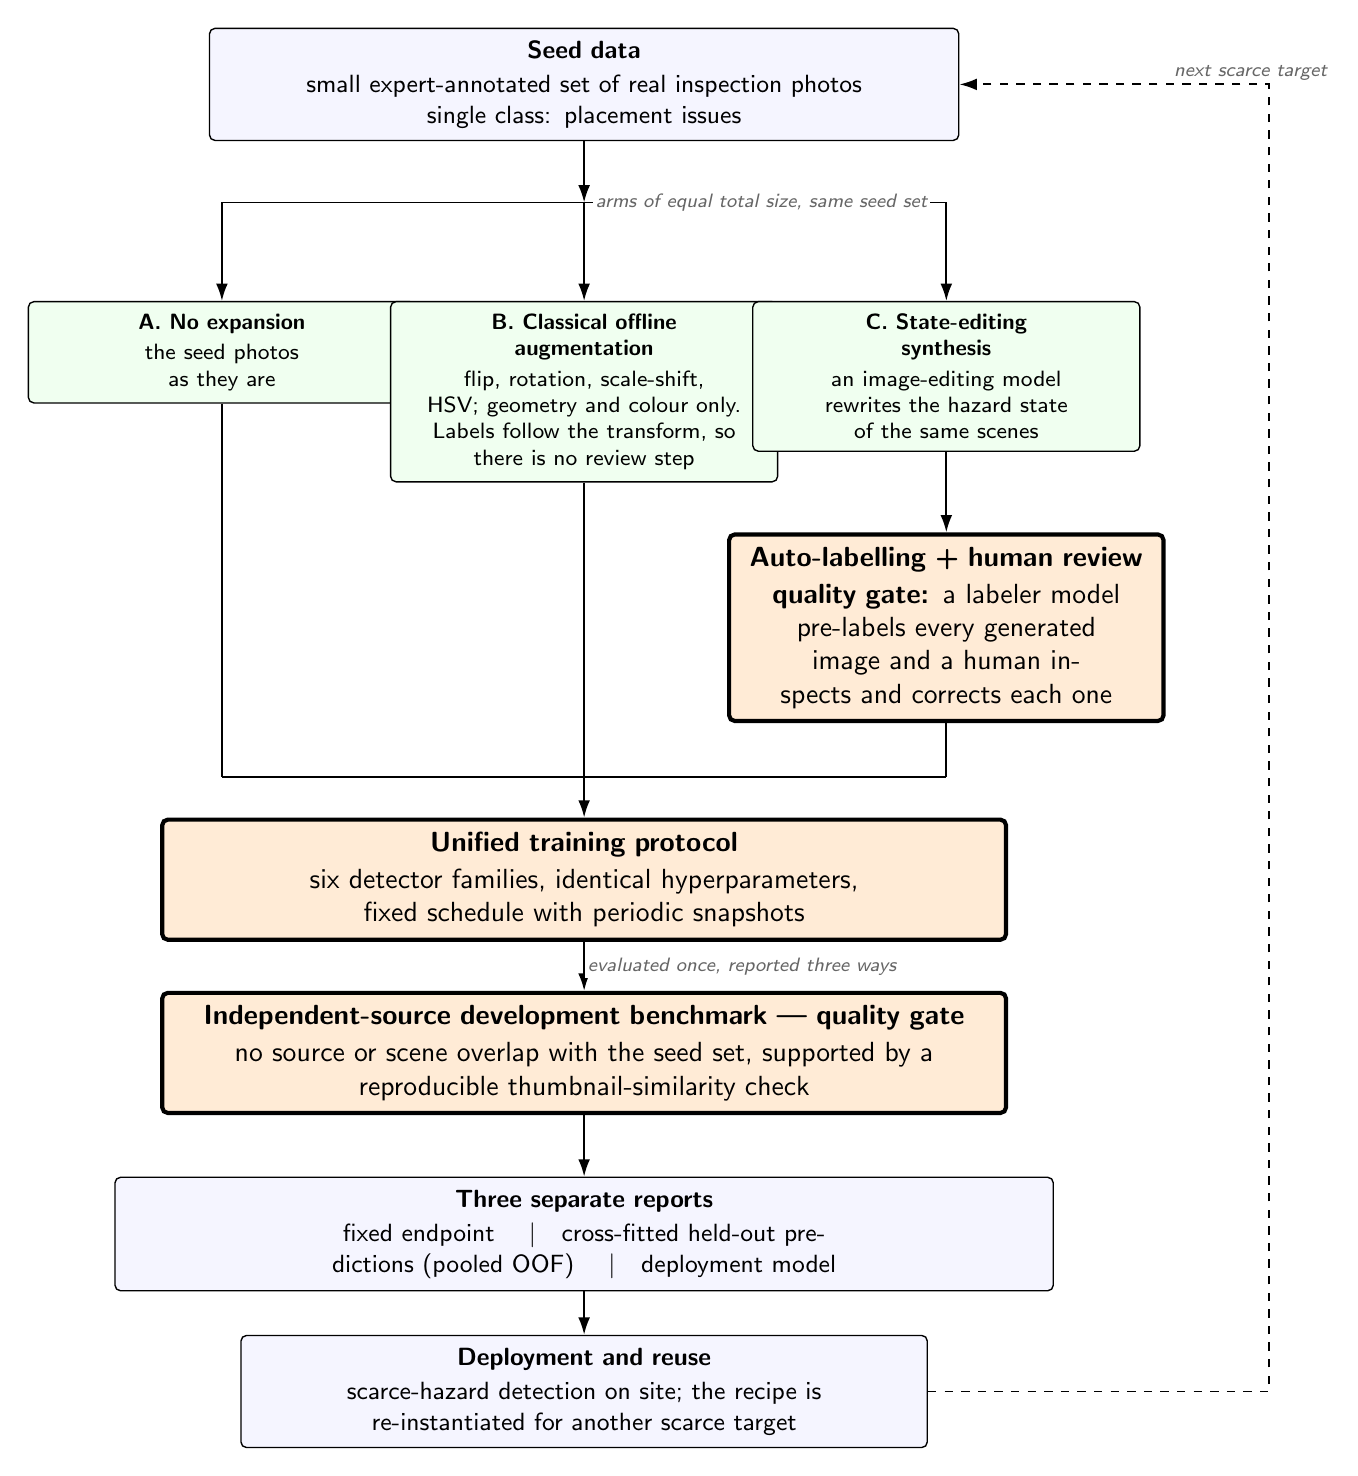
\begin{tikzpicture}

  % ---------- stage 1: seed ----------
  \node[box, text width=9.2cm] (seed) at (4.6, 0)
    {\textbf{Seed data}\\[1.5pt]
     small expert-annotated set of real inspection photos\\
     single class: placement issues};

  % ---------- stage 2: three same-source expansion arms ----------
  \coordinate (split) at (4.6, -1.5);
  \node[arm, text width=4.6cm] (armA) at (0, -2.75)
    {\textbf{A. No expansion}\\[1.5pt] the seed photos\\ as they are};
  \node[arm, text width=4.6cm] (armB) at (4.6, -2.75)
    {\textbf{B. Classical offline\\ augmentation}\\[1.5pt]
     flip, rotation, scale-shift,\\
     HSV; geometry and colour only.\\
     Labels follow the transform, so\\
     there is no review step};
  \node[arm, text width=4.6cm] (armC) at (9.2, -2.75)
    {\textbf{C. State-editing\\ synthesis}\\[1.5pt]
     an image-editing model\\
     rewrites the hazard state\\
     of the same scenes};

  \draw[flow] (seed.south) -- (split);
  \draw[flow] (split) -| (armA.north);
  \draw[flow] (split) -| (armB.north);
  \draw[flow] (split) -| (armC.north);
  \node[tag, anchor=west] at ([xshift=3pt]split)
    {arms of equal total size, same seed set};

  % ---------- stage 3: labelling loop, arm C only ----------
  \node[gate, text width=5.2cm] (review) at (9.2, -6.9)
    {\textbf{Auto-labelling + human review}\\[1.5pt]
     \textbf{quality gate:} a labeler model pre-labels every
     generated image and a human inspects and corrects each one};
  \draw[flow] (armC.south) -- (review.north);

  % ---------- stage 4: unified training and cross-fitted evaluation ----------
  \coordinate (bus) at (4.6, -8.6);
  \node[gate, text width=10.4cm] (train) at (4.6, -10.1)
    {\textbf{Unified training protocol}\\[1.5pt]
     six detector families, identical hyperparameters,\\
     fixed schedule with periodic snapshots};
  \node[gate, text width=10.4cm] (dev) at (4.6, -12.3)
    {\textbf{Independent-source development benchmark --- quality gate}\\[1.5pt]
     no source or scene overlap with the seed set, supported by a\\
     reproducible thumbnail-similarity check};
  \node[box, text width=11.6cm] (report) at (4.6, -14.6)
    {\textbf{Three separate reports}\\[1.5pt]
     fixed endpoint \quad$\vert$\quad cross-fitted held-out predictions (pooled OOF)
     \quad$\vert$\quad deployment model};

  % The three branches merge into one horizontal bus, then a single arrow enters training.
  \draw[plain] (armA.south) -- (0, -8.8);
  \draw[plain] (armB.south) -- (4.6, -8.8);
  \draw[plain] (review.south) -- (9.2, -8.8);
  \draw[plain] (0, -8.8) -- (9.2, -8.8);
  \draw[flow] (4.6, -8.8) -- (train.north);
  \draw[flow] (train.south) -- node[tag, right] {evaluated once, reported three ways}
    (dev.north);
  \draw[flow] (dev.south) -- (report.north);

  % ---------- stage 5: deployment and reuse ----------
  \node[box, text width=8.4cm] (reuse) at (4.6, -16.6)
    {\textbf{Deployment and reuse}\\[1.5pt]
     scarce-hazard detection on site; the recipe is\\
     re-instantiated for another scarce target};
  \draw[flow] (report.south) -- (reuse.north);
  \draw[aux] (reuse.east) -- (13.3, -16.6) -- (13.3, 0) -- (seed.east)
    node[tag, pos=0.06, above] {next scarce target};

\end{tikzpicture}
\end{document}
